\documentclass[a4paper,12pt]{article}
\usepackage{graphicx}
\usepackage[UTF8]{ctex}
\usepackage{fontspec}
\usepackage{booktabs}
\usepackage{float}%浮动体
\usepackage{amsmath,amssymb}
\usepackage{fancyhdr}
%\usepackage{xcolor}
\usepackage{colortbl}
\usepackage{geometry}
\geometry{top=2cm,bottom=2cm,left=1cm,right=1cm}
\begin{document}
	\begin{figure}[H]
	\begin{center}
		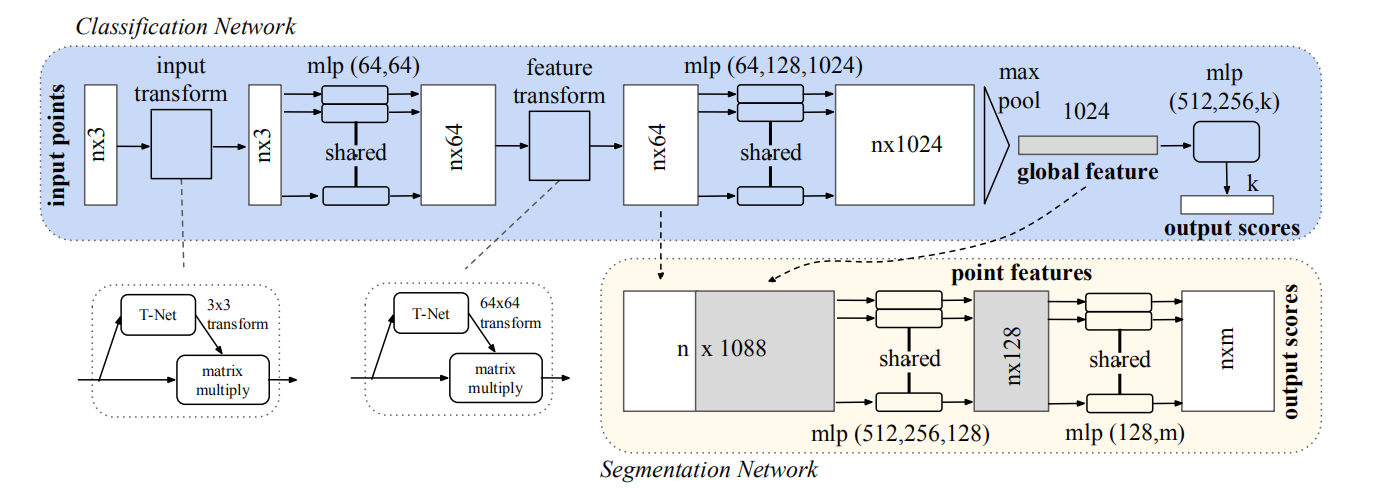
\includegraphics[width=0.9\textwidth]{img/PointNet.png} 
		\caption{PointNet}
	\end{center}
\end{figure}

	\begin{figure}[H]
	\begin{center}
		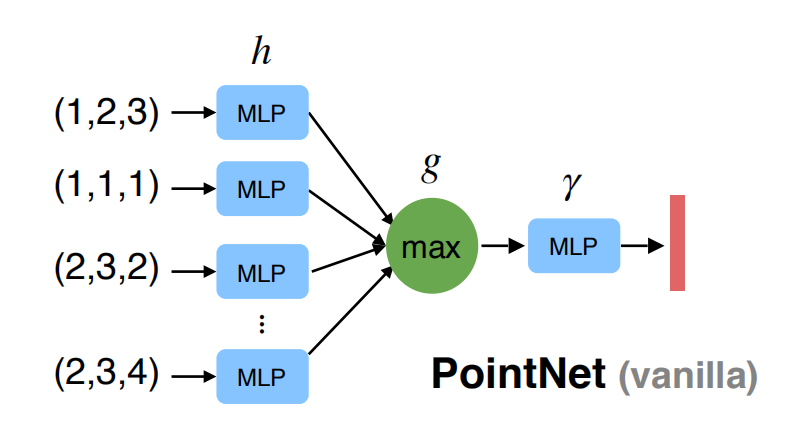
\includegraphics[width=0.5\textwidth]{img/symmetry.png} 
		\caption{PointNet}
	\end{center}
\end{figure}

\begin{itemize}
	\item 排列不变性:对称函数
	$$
	f\left(x_{1}, x_{2}, \ldots, x_{n}\right) =\gamma \circ g\left(h\left(x_{1}\right), \ldots, h\left(x_{n}\right)\right)
	$$
	$$
	\left|f(S)-\gamma\left(\underset{x_{i} \in S}{\operatorname{MAX}}\left\{h\left(x_{i}\right)\right\}\right)\right|<\epsilon
	$$
	可以任意逼近所有连续的集合函数(没找到证明材料)。
	\item 旋转不变性:Spatial Transformer Network,并在loss\_function上加上这个约束 $L_{r e g}=\left\|I-A A^{T}\right\|_{F}^{2}$
	\item  点与点之间存在影响:将全局特征与每个点特征叠加
\end{itemize}
\paragraph{分类任务}
使用T-Net网络对输入特征进行旋转,然后使用MLP使每个点的特征增加,随后对特征进行旋转。这里PointNet用的MLP是卷积核,将每个点都进行特征提取,使其channel变多,本质是信息的冗余。随后使用Maxpool,提取整体特征。最后使用MLP(Linear),进行分类。
\paragraph{语义分割} 在分类任务提取整体特征的基础上,将整体特征重复n次,然后和每个点的特征叠加起来,最后还是一连串的MLP(卷积)+softmax


\end{document}